\documentclass[newPxFont,numfooter,sectionpages]{beamer}
\usepackage[utf8]{inputenc}
\usepackage[T2A]{fontenc}
\usepackage[russian]{babel}
\usepackage{eufrak}
\usetheme{sthlm}
\usepackage{pgfplots}
\usepackage{cancel}

\usepackage{multirow}
\usepackage[normalem]{ulem}
\useunder{\uline}{\ul}{}

\title{Вычислительно эффективные алгоритмы решения прямой и обратной задач динамики}
\subtitle{}
%\date{\today}
\author{\texttt{Artemov K.}}
%\institute{ITMO University}}

\begin{document}

\maketitle


\begin{frame}{Содержаине}
	% For longer presentations use hideallsubsections option
	\tableofcontents[hideallsubsections]
	\begin{itemize}
		\item 
		Что есть прямая и обратная задачи динамики
		\item Как оценивается эффектиность алгоритмов
		\item Уравнения движения
		\item Алгоритмы основанные на уравнениях Лагранжа, Ньютона-Эйлера, Аппеля и Кейна
		\item Обзор некоторых алгоритмов
		
	\end{itemize}	
\end{frame}

\begin{frame}{Прямая и обратная задачи динамики}
	\begin{minipage}{0.45\textwidth}
		\begin{center}
			\cOrange{\underline{Прямая задача динамики:}}
			
			\cOrange{Заданы:} обобщенные силы/моменты;
			
			\cOrange{Найти:} определить траекторию движения.
			
			\begin{equation*}
			\ddot q = \phi(q, \dot q, \tau)
			\end{equation*}
		\end{center}
	
	\end{minipage}
	\hfill
	\begin{minipage}{0.45\textwidth}
		\begin{center}
			\cOrange{\underline{Обратная задача динамики:}}
			
			\cOrange{Задана:} траектория движения;
			
			\cOrange{Найти:} обобщенные силы/моменты.
			
			\begin{equation*}
			\tau = \phi(q, \dot q, \ddot q)
			\end{equation*}		
		\end{center}
	
	\end{minipage}
	\begin{center}
	где $\tau$ -- вектор обобщенных сил/моментов робота, $q, \dot q$ и $\ddot q$ -- векторы положения, скорости и ускорения
	\end{center}
\end{frame}

\begin{frame}{Оценка эффективности алгоритмов}
	\cOrange{Временная сложность алгоритмов:}
	\begin{itemize}
		\item $O(1)$ -- постоянное время;
		\item $O(n)$ -- линейное время;
		\item $O(n^2)$ -- квадратичное время;
		\item и др.
	\end{itemize}
	\cOrange{Вычислительная сложность алгоритмов:}
	\begin{itemize}
	\item количество сложений;
	\item количество умножений.
	\end{itemize}
\end{frame}

\begin{frame}{Уравнения движения}
\begin{itemize}
	\item \cOrange{уравнение в конфигурационном пространстве:}
	\begin{center}
		$M(q) \ddot q + C(q, \dot q)\dot q + G (q) = \tau$	
	\end{center}
	где $q, \dot q$ и $\ddot q$ -- положение, скорость и ускорение звена робота, $\tau$ -- силы/моменты приложенные к звену, $M(q)$ -- тензор инерции, $C(q, \dot q)$ -- матрица Кориолисовых и центробежных сил, $G(q)$ -- вектор гравитации;
	
	\item \cOrange{уравнение в операционном пространстве:}
	\begin{center}
		$\Lambda(x) \ddot x + \mu (x, \dot x) + \rho (x) = f$
	\end{center}		
	где $x$ -- положение схвата, $\dot x$ -- скорость схвата, $f$ -- действующие силы на схват, $\Lambda(x)$ -- матрица инерции в операционном пространстве, $\mu(x, \dot x)$ -- содержит Кориолисовы и центробежные составляющие, $\rho(x)$ -- вектор гравитации.
\end{itemize}
\end{frame}

\begin{frame}{Уравнения и алгоритмы}
\begin{table}[]
	\centering
	\caption{Алгоритмы основанные на уравнениях Эйлера-Лагранжа}
	\label{my-label}
	\begin{tabular}{|l|l|r|r|c|}
		\hline
		\multicolumn{1}{|c|}{\multirow{2}{*}{\begin{tabular}[c]{@{}c@{}}Форма\\ уравнений\end{tabular}}} & \multicolumn{1}{c|}{\multirow{2}{*}{\begin{tabular}[c]{@{}c@{}}Авторы\\ алгоритма\end{tabular}}} & \multicolumn{2}{c|}{Число операций} & \multirow{2}{*}{\begin{tabular}[c]{@{}c@{}}Прямая\\ задача\end{tabular}} \\ \cline{3-4}
		\multicolumn{1}{|c|}{} & \multicolumn{1}{c|}{} & \multicolumn{1}{c|}{*} & \multicolumn{1}{c|}{+} &  \\ \hline
		\multirow{4}{*}{Лагранж} & Uicker/Kahn & 66271 & 51548 & + \\ \cline{2-5} 
		& \begin{tabular}[c]{@{}l@{}}Vukobratovic/\\ Potconjak\end{tabular} & 37189 & 5652 & + \\ \cline{2-5} 
		& Hollerbach 3x3 & 2195 & 1719 & - \\ \cline{2-5} 
		& Renaud & 992 & 776 & + \\ \hline
	\end{tabular}
\end{table}
\end{frame}

\begin{frame}{Уравнения и алгоритмы}
\begin{table}[]
	\centering
	\caption{Алгоритмы основанные на уравнениях Ньютона-Эйлера}
	\label{my-label}
	\begin{tabular}{|c|l|r|r|c|}
		\hline
		\multirow{2}{*}{\begin{tabular}[c]{@{}c@{}}Форма\\ уравнений\end{tabular}} & \multicolumn{1}{c|}{\multirow{2}{*}{\begin{tabular}[c]{@{}c@{}}Авторы\\ алгоритма\end{tabular}}} & \multicolumn{2}{c|}{Число операций} & \multirow{2}{*}{\begin{tabular}[c]{@{}c@{}}Прямая\\ задача\end{tabular}} \\ \cline{3-4}
		& \multicolumn{1}{c|}{} & \multicolumn{1}{c|}{*} & \multicolumn{1}{c|}{+} &  \\ \hline
		\multirow{5}{*}{Ньютон-Эйлер} & \begin{tabular}[c]{@{}l@{}}Vukobratovic/\\ Stepanenko\end{tabular} & 2907 & 2068 & + \\ \cline{2-5} 
		& Walker/Orin & 1771 & 1345 & + \\ \cline{2-5} 
		& Wang/Ravani & 1659 & 1252 & + \\ \cline{2-5} 
		& \begin{tabular}[c]{@{}l@{}}Luh/Walker/\\ Paul\end{tabular} & 792 & 662 & - \\ \cline{2-5} 
		& \begin{tabular}[c]{@{}l@{}}Balafoutis/\\ Patel/Misra\end{tabular} & 489 & 420 & - \\ \hline
	\end{tabular}
\end{table}
\end{frame}

\begin{frame}{Уравнения и алгоритмы}
	\begin{table}[]
		\centering
		\caption{Алгоритмы основанные на других уравнениях}
		\label{my-label}
		\begin{tabular}{|l|l|c|r|c|}
			\hline
			\multicolumn{1}{|c|}{\multirow{2}{*}{\begin{tabular}[c]{@{}c@{}}Форма\\ уравнений\end{tabular}}} & \multicolumn{1}{c|}{\multirow{2}{*}{\begin{tabular}[c]{@{}c@{}}Авторы\\ алгоритма\end{tabular}}} & \multicolumn{2}{c|}{Число операций} & \multirow{2}{*}{\begin{tabular}[c]{@{}c@{}}Прямая\\ задача\end{tabular}} \\ \cline{3-4}
			\multicolumn{1}{|c|}{} & \multicolumn{1}{c|}{} & * & \multicolumn{1}{c|}{+} &  \\ \hline
			Аппель & Попов & \multicolumn{1}{r|}{2929} & 2500 & + \\ \hline
			Кейн & Ma/Xu & \multicolumn{1}{r|}{1020} & 851 & - \\ \hline
		\end{tabular}
\end{table}
\end{frame}

\begin{frame}{Алгоритм Uiker и Kahn}

Уравнения динамики для робота с $n$ степенями свободы:

\begin{align*}\label{eq1}
P_i &= \sum_{j=i}^{n}
\left(
\sum_{k=1}^{j}
\left[
tr(\frac{\partial W_j}{\partial q_i} J_j \frac{\partial W_j^T}{\partial q_k})
\right] \ddot q_k 
\right.&\\
&+
\left.
\sum_{k=1}^{j} \sum_{l=1}^{j} 
\left[
tr(\frac{\partial W_j}{\partial q_i} J_j \frac{\partial^2 W_j^T}{\partial q_k \partial q_l})\dot q_k \dot q_l
\right]
-m_j \vec{q^T} \frac{\partial W_j}{\partial q_i} r_{jo}
\right)
\end{align*}
где $P_i$ -- сила/момент привода, $W_i$ -- матрица трансформации от базовой к локальной системе координат $i$-ого звена, $J_i$ -- матрица инерции $i$-ого звена в локальной системе координат, $m_i$ -- масса звена $i$, $r_{j0}$ -- вектор от центра масс звена $i$ к началу базовой системы координат, выраженный в локальной системе координат звена $i$, $\vec g$ -- вектор гравитации
\end{frame}

\begin{frame}{Алгоритм Uiker и Kahn (продолж.)}
	
	Матрица $W_i$ выражается, как:
	\begin{equation*}
	W_i = A_1^0 A_2^1 ... A_i^{i-1}
	\end{equation*}
	где $A_i^{i-1}$ -- матрица трансформации $4 \times 4$ из $i-1$ в $i$ системаму координат
	
	\begin{figure}[H]
		\center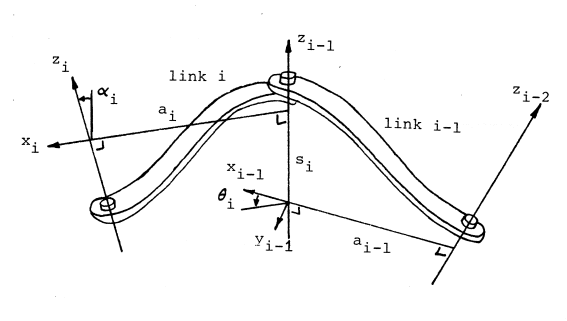
\includegraphics[width=0.7\linewidth]{1.png}
		\caption{Оси координат двух соседних звеньев}
		\label{fig:scr1}
	\end{figure}
\end{frame}

\begin{frame}{Алгоритм Uiker и Kahn (продолж.)}
	Формулы для вычисления частных производных матриц $W_i$:
	\begin{align*}
	\frac{\partial W_i}{\partial q_k} &= W_{k-1} \frac{\partial A_k}{\partial q_k} ^k W_i, &(k \le i)\\
	\frac{\partial^2 W_i}{\partial q_k \partial q_l} 
	&= W_{k-1} \frac{\partial A_k}{\partial q_k} ^k W_{l-1}\frac{\partial A_l}{\partial q_l} ^l W_i, &(k < l \le i) \\
	&= W_{k-1} \frac{\partial^2 A_k}{\partial q_k^2} ^k W_i, &(k = i)
	\end{align*}
\end{frame}

\begin{frame}{Алгоритм Uiker и Kahn (продолж.)}
	Алгоритм -- нерекурсивный.
	
	Решение прямой задачи динамики:
	\begin{equation*}
		P = H(q) \ddot q + \dot q^T C(q) \dot q + g(q)
	\end{equation*}
	Решение обратной задачи динамики:
	\begin{equation*}
		\ddot q = H(q)^{-1}(\dot q^T C(q) \dot q + g(q)) - P
	\end{equation*}
	Вычислительная сложность:
	\begin{itemize}
		\item количество сложений порядка $n^4$;
		\item количество умножений порядка $n^4$.
	\end{itemize}
\end{frame}

\begin{frame}{Алгоритм Hollerbach}

Для вычисления частных производных в уравнении:
\begin{equation*}
\label{eq6}
P_i = 
\sum_{j=i}^{n}
\left[
tr(
\frac{\partial W_j}{\partial q_i} ^i W_j J_j \ddot W_j^T
)
- m_j \vec g^T \frac{\partial W_j}{\partial q_i} ^i W_j r_{i0}
\right]
\end{equation*} 
применены рекурсивные отношения:
\begin{align*}
W_j &= W_{j-1} A_j^{j-1}\\
\dot W_j &= \dot W_{j-1} A_j^{j-1} + W_{j-1} \frac{\partial A_j^{j-1}}{\partial q_j} \dot q_j\\
\ddot W_j &= \ddot W_{j-1} A_j^{j-1} + 2 \dot W_{j-1}
\frac{\partial A_j^{j-1}}{\partial q_j} \dot q_j +
W_{j-1} \frac{\partial^2 A_j^{j-1}}{\partial q_j^2} \dot q_j^2 +
W_{j-1} \frac{\partial A_j^{j-1}}{\partial q_j} \ddot q_j 
\end{align*}

\end{frame}

\begin{frame}{Алгоритм Hollerbach (продолж.)}
	
Если представить уравнение движения в следующей форме:
\begin{equation*}
P_i = tr(\frac{\partial W_i}{\partial q_i}) D_i -
\vec{g}^T \frac{\partial W_i}{\partial q_i} c_i
\end{equation*}
где 
\begin{align*}
D_i &= J_i \ddot W_i^T + A_{i+1}^{i} D_{i+1}\\
c_i &= m_i r_{i0} + A_{i+1}^{i} c_{i+1}.
\end{align*}

Угловое ускорение $\ddot W_i^T$ вычисляется в прямой рекурсии от базы к схвату. $D_i$ и $c_i$ вычисляются в обратной рекурсии от схвата к базе.

Таим образом, полученные соотношения позволяют достичь $30n-592$ операций умножения и $675n - 464$ операций сложения.
\end{frame}

%NEWTON

\begin{frame}{Алгоритм Vukobratovic и Stepanenko}
	Алгоритм позволяет рассчитывать инверсную динамику кинематических цепочек с фиксировнной базой.
	
	Вычисления производятся в четыре этапа:
	\begin{itemize}
		\item Этап 1:
		Вычисляется скорость и ускорения для каждого звена, начиная с известных скорости и ускорения базы и заканчивая схватом
		\begin{equation*}
		v_i = ^iX_{p(i)} v_{p(i)} + \Phi_i \dot q_i, (v_0 = 0),
		\end{equation*}
		
		где $v_i$ -- скорость звена $i$, $\Phi_i$ -- тип сочленения $j$, и $\dot q_i$ -- вектор скорости.
		
		\end{itemize}	

\end{frame}
\begin{frame}{Алгоритм Vukobratovic и Stepanenko (продолж.)}
		Ускорение:
		\begin{equation*}
		a_i = ^iX_{p(i)} a_{p(i)} + \Phi_i \ddot q_i ++ \dot\Phi_i \dot q_i, (a_0 = 0), 
		\end{equation*}
		
		где $a_i$ -- ускорение звена $j$, $\ddot q_i$ -- вектор ускорения обобщенных переменных сочленения $j$.
		
		Для того, чтобы учесть влияние ускорения свободного поения на систему, возможно инициализировать $a_0 = -g$ вместо нуля. В этом случае $a_i$ будет характеризовать ускорение звена $i$ с учетом ускорения свободного подения.
	
\end{frame}
\begin{frame}{Алгоритм Vukobratovic и Stepanenko (продолж.)}
		\begin{itemize}
		\item Этап 2:
На этом этапе рассчитываются силы, которые нужно приложить к звену, чтобы оно приобрело расчитанное на Этапе 1 ускорение
\begin{equation*}
f^a_i = I_i a_i + v_i \times I_i v_i,
\end{equation*}

где $I_i$ вектор инерции звена $i$, $f^a_i$ -- равнойствующая сила на звено $i$.

\end{itemize}
\end{frame}
\begin{frame}{Алгоритм Vukobratovic и Stepanenko (продолж.)}
	\begin{itemize}
		\item Этап 3:
		Вычисляется вектор сил через каждое из звеньев
		\begin{equation*}
		f_i = f^a_i - ^iX_{p(i)} f^e_i + \Sigma_{j \in c(i)} ^iX_{p(i)} f_j,
		\end{equation*}
		где $f_i$ -- сила передающаяся через звено $j$, $f^e_i$ -- сумма всех внешних сил, дейстующих на звено $i$, $c(i)$ множество потомков звена $i$, $i = n,...,1$.
		
		$f^e_i$ может представлять собой пружины, демпферы, контакты с внешней средой, а также ускорение свободного подения, если он не задан на Этапе 2 и прочее, т.е. заранее известна.
		
		\item Этап 4:
		Вычисляются обобщенные моменты/силы
		
		\begin{equation*}
		\tau_i = \Phi_i^T f_i
		\end{equation*}
	\end{itemize}
\end{frame}


\begin{frame}{Рекурсивный алгоритм НЬютона-Эйлера}
	\begin{minipage}{0.45\textwidth}
	\begin{center}
	\begin{figure}[H]
	\center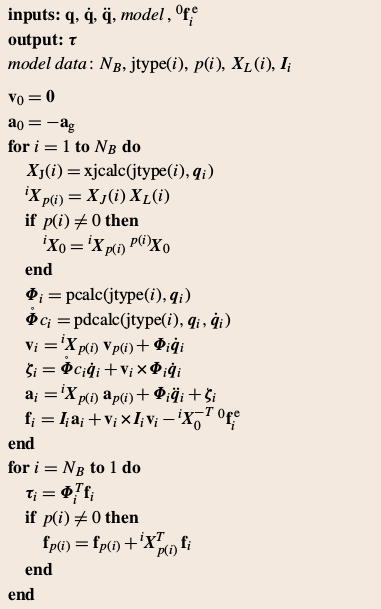
\includegraphics[width=1\linewidth]{555.png}
	\end{figure}
	\end{center}
	
\end{minipage}
\hfill
\begin{minipage}{0.45\textwidth}
Входные данные: траектория движения, модель робота, внешние силы;

Выходными данные: моменты приводов;

Функция \cOrange{jtype} -- возвращает тип звена;

Функиця \cOrange{xjtype} -- матрицу трансформации для указанного типа звена;

Функции \cOrange{pcalc} и \cOrange{pdcalc} вычисляют $\Phi_i$ и $\dot Phi_i$;

$X$ -- матрица трансформации.
\end{minipage}

\end{frame}

\begin{frame}{Алгоритмы основанные на уравнениях Аппеля}
Динамика механизма описывается уравнениями Гиббса-Аппеля:
\begin{equation*}
\frac{\partial G}{\partial \ddot q_i} = Q_i, (i=1,...,n)
\end{equation*}
где $G$ -- функция "энергии ускорения", $Q_i$ -- обобщенная сила.

Функция "энергии ускорения" может быть выражена как сумма:
\begin{equation*}
G = \sum_{i=1}^n G_i
\end{equation*}
где $G_i$ -- функция Гиббса для звена $i$, которая, в свою очередь, определется из выражения:
\begin{equation*}
G_i = \frac{1}{2} m_i w_i^2 + \frac{1}{2} \epsilon_i^T J_i \epsilon_i + 2 (\omega_i \times J_i \omega_i) \epsilon_i
\end{equation*}

\end{frame}

\begin{frame}{Алгоритмы основанные на уравнениях Аппеля (продолж.)}

	Подставляя в последнее выражения рекурсивные отношения для кинематики робота, получаем динамическую модель робота в форме:
	
	\begin{equation*} \label{eq8}
	H(q) \ddot q + h_c (q, \dot q) = Q
	\end{equation*}
	где $Q = P - g(q)$ -- вектор обобщенных сил.
	\begin{equation*}
	H(q) \ddot q + h (q, \dot q) = P
	\end{equation*}
	где $h (q, \dot q) = h_c (q, \dot q) + g(p)$.
	
	Этот алгоритм позволяет решать как прямую, так и обратную задачи динамики. Вычислительная сложность: $\frac{7}{3} n^3 + 27 n^2 + \frac{722}{3} n + 9$ -- умножений, $\frac{10}{3} n^3 + \frac{43}{2} n^2 + \frac{931}{6} n + 6$ -- сложений.
\end{frame}


\begin{frame}{Алгоритмы основанные на уравнениях Кейна}
	Считается, что робот состоит из $n$ соединеных твердых тел, каждое из которых имеет по 6 степеней свободы. Относительная ориентация соседних звеньев описывается следующими четырьмя параметрами Эйлера:
	
	\begin{align*}
	\epsilon_{il} &= e_{il} sin (\frac{q_i}{2}), (l=1,2,3)\\
	\epsilon_{i4} &= e_{i4} cos (\frac{q_i}{2}). 
	\end{align*}
	где $e_i = (e_{i1}, e_{i2}, e_{i3})$ -- единичный вектор на оси, вокруг которой $i-1$ локальная система координат переходит в $i$ в результате вращения, $q_i$ -- угол, $e_{i4} = 1$. Можно показать, что параметры Эйлера эквивалентны формеле Родрига, когда сочленения с одной степенью свободы связаны. 
\end{frame}



\begin{frame}{Алгоритмы основанные на уравнениях Кейна (продолж.)}

Можно показать, что параметры Эйлера эквивалентны формеле Родрига, когда сочленения с одной степенью свободы связаны. 

\begin{equation*}
r' = r + 2 sin (\frac{q_i}{2}) e_i \times (e_i \times r) + 2 sin (\frac{q_i}{2}) cos (\frac{q_i}{2}) (e_i \times r)
\end{equation*}
где $r$ -- вектор до вращения, $r'$ -- вектор после вращения на угол $q_i$ вокруг оси $e_i$. Сделав замену $\epsilon_i =e_i sin (\frac{q_i}{2}) $ и $\epsilon_{i4} = cos  (\frac{q_i}{2})$, получим:
\begin{equation*}
r' = r + 2 \epsilon_i \times (\epsilon_i \times r) + 2 sin (\frac{q_i}{2}) \epsilon_{i4} (\epsilon_i \times r)
\end{equation*}

\end{frame}

\begin{frame}{Алгоритмы основанные на уравнениях Кейна (продолж.)}
	
	Кинематические соотношения в этом алгоритме состоят из  выражения для скоростей и ускорений звеньев в терминах параметров Эйлера:
	
	\begin{equation*}
	\omega_i = \sum_{k=1}^{i} \omega'_i
	\end{equation*}
	где $\omega_i$ -- угловая скорость звена $i$ относительно базовой системы координат, $\omega'_k$ -- относительная угловая скорость звена $k$ относительно звена $k-1$. Это соотношение можно переписать в рекурсивной форме:
	
	\begin{equation*}
	\omega_i = \omega_{i-1} + \omega'_i
	\end{equation*}
	
	Несложно заметить, что это уравнение совпадает с ранее рассмотренным. 
\end{frame}

\begin{frame}{Алгоритмы основанные на уравнениях Кейна (продолж.)}
	
Несмотря на постоянный рост мощности компьютеров, требование высокой вычислительной эффективности уравнений динамики остается критичным. Это объясняется тем, что:
\begin{itemize}
\item во-первых, в системах управления роботов используются как правило относительно медленные процессоры, и для решения уравнений динамики в реальном времени необходимы эффективные алгоритмы расчета
\item во-вторых, сложность механических структур современных роботов (параллельных, с избыточными степенями подвижности, так называемых роботов-гуманоидов) требует эффективных методов расчета динамики для задач их моделирования и управления.
\end{itemize}
\end{frame}

\begingroup
\setbeamercolor{background canvas}{bg=\cnDarkGrey}
\begin{frame}[plain]
	
	\centering{\cGrey{\LARGE{СПАСИБО ЗА ВНИМАНИЕ!}}}
	\begin{center}
	\cGrey{\texttt{Artemov K.}}\\
	\cGrey{ITMO University}\\
	\cGrey{dec. 2016}
\end{center}	
\end{frame}
\endgroup
\end{document}
